\chapter{Feedback}\label{c:feedback}
\section{Uses of Feedback}

disturbance rejection
parameter sensitivity
command tracking
\section{Anatomy of Feedback Control}

\begin{figure}[hbt]
\centering
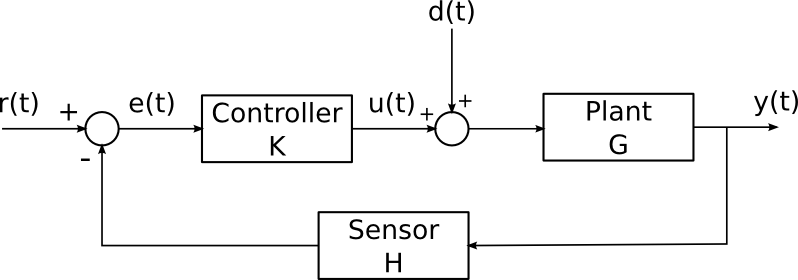
\includegraphics[width=\FigWidth\textwidth]{feedback.png}
\caption{Canonical feedback control system block diagram.}
\label{f:fdbk}
\end{figure}

process
disturbance
actuator
plant 
controller
sensor


\section{PID Control}

\section{Assessing Stability}

\section{Assessing Performance}

This chapter is about \gls{feedback}s.
